Краткое напоминаю, что в конце предыдущей лекции мы изучали реверсивные
преобразователи.
Под реверсией понимают изменение чего-либо на противопожное.
Если иметь ввиду двигатель, то реверс означает вращение в другую сторону.
Напряжение реверсируется даже в нереверсивном преобразователе.
Для того чтобы ток был реверсивным нужно как минимум два комплекта вентилей.
В классификации реверсивных преобразователей в первом классе были
преобразователи с одной группой вентилей. Переключение тока происходило
посредством переключения полюсов нагрузки с полюсами питания.
В истинно реверсивных преобразователях существуют две группы вентилей.

\subsection{перекрестрая схема}
исторически самая первая.

\begin{figure}[H]
\begin{circuitikz}\draw
  (0,3.5) to[L] ++ (0,-1)
  to[Ty,l_=$\begin{array}{c}
      \textcyrillic{1я группа}\\
      \textcyrillic{вентилей}\end{array}$] ++ (0,-1.5)
  -- ++ (1,0)
  (0,3.5) -- ++ (1,0)
  to[L] ++ (0,-1)
  to[Ty,-*] ++ (0,-1.5)
  -- ++ (1,0)
  (1,3.5) -- ++ (1,0)
  to[L] ++ (0,-1)
  to[Ty,-*] ++ (0,-1.5)
  % уравнительный реактор Ур1
  -- ++ (1.5,0)
  to[L,l={$\textcyrillic{Ур1}$}] ++ (0,1)
  -- ++ (1.5,1.5)
  -- ++ (1,0)
  % 2я группа вентилей
  to[L] ++ (0,-1)
  to[Ty,-*] ++ (0,-1.5)
  -- ++ (1,0)
  (6,3.5) -- ++ (1,0)
  to[L] ++ (0,-1)
  to[Ty,-*] ++ (0,-1.5)
  -- ++ (1,0)
  (7,3.5) -- ++ (1,0)
  to[L] ++ (0,-1)
  to[Ty,l=$\begin{array}{c}
      \textcyrillic{2я группа}\\
      \textcyrillic{вентилей}\end{array}$] ++ (0,-1.5)
  % уравнительный реактор Ур2
  (6,1) -- ++ (-1.5,0)
  to[L,l_={\textcyrillic{Ур2}}] ++ (0,1)
  -- ++ (-1.5,1.5)
  -- ++ (-1.5,0)
  % мотор
  (1,1) -- ++ (0,-1.5)
  -- ++ (2.5,0)
  (4,-0.5) circle (0.5 cm)
  (4,-0.5) node {M}
  (4.5,-0.5) -- ++ (2.5,0)
  -- ++ (0, 1.5)
  % первичная сторона
  (3, 5) to[L] ++ (0,-1)
  -- ++ (1,0)
  (4, 5) to[L] ++ (0,-1)
  -- ++ (1,0)
  (5, 5) to[L] ++ (0,-1)
  % core
  [thick] (0,3.74) rectangle (8,3.77)
  ;\end{circuitikz}
\caption{перекрестная схема реверсивного преобразователя}
\end{figure}

$\textcyrillic{Ур1}$ и $\textcyrillic{Ур1}$ -- уравнительные реакторы.
Силовые индуктивности рисуются как
\begin{circuitikz}\draw
  (0,0.8) -- ++ (0,-0.8)
  (0.5,0) arc(0:270:0.5)
  (0.5,0) -- ++ (-0.5,0)
  (0,-0.5) -- ++ (0,-0.3)
  ;\end{circuitikz}
 или как  
\begin{circuitikz}\draw
(0,0.8) --++ (0,-0.3)
(-0.5,0) arc(-180:90:0.5)
(-0.5,0)--++(0.5,0)
(0,0)--++(0,-0.8)  
  ;\end{circuitikz}

\begin{figure}[H]
  \begin{circuitikz}\draw
    (0,1) to[L,-*] ++(2,0)
    to[L] ++(2,0)
    --++(0,1)
    to[Ty,*-] ++(-1.3,0)
    --++(-1.4,0)
    to[Ty,*-*] ++(-1.3,0)
    --++(0,-1)
    (4,2)--++(0,1)
    to[Ty,*-*]++(-1.3,0)
    --++(-1.4,0)
    to[Ty,-*]++(-1.3,0)
    --++(0,-1)
    (4,3)--++(0,1)
    to[Ty]++(-1.3,0)
    to[short,-*]++(-0.7,0)
    --++(-0.7,0)
    to[Ty]++(-1.3,0)
    --++(0,-1)
    %LLL
    (1.3,2)--++(0,2)
    to[L]++(0,1.3) %La'
    --++(-0.4,0)
    --++(0,1.7)
    --++(1.8,0)
    (2,4) to[L]++(0,1.3) %Lb
    --++(-0.4,0)
    --++(0,1.5)
    --++(-0.3,0)
    (1.3,5.5) to[L]++(0,1.3) %La''

    (1.3,5.5)--++(0.7,0)
    to[L,*-]++(0,1.3) %Lb''
    (2.7,3)--++(0,1)
    to[L]++(0,1.3) %Lc'
    --++(-0.4,0)
    --++(0,1.5)
    --++(-0.3,0)
    (2,5.5)--++(0.7,0)
    to[L,*-]++(0,1.3) %Lc''
    --++(0,0.2)
    %мотор
    (2,1)--++(0,-0.5)
    (2,0) circle (0.5cm)
    (2,0) node {M}
    (2,-0.5)--++(0,-0.5)
    --++(2.3,0)
    --++(0,6.5)
    --++(-1.6,0)
    %core
    [thick] (0.9,7.2) rectangle (3.1,7.22)
    % первичная сторона
    (1.3,7.4) to[L]++(0,1.3)
    (2,7.4) to[L]++(0,1.3)
    (2.7,7.4) to[L]++(0,1.3)
    (1.3,7.4) -- (2.7,7.4)
    ;
    % стрелки
%    \draw[<-] (0.2,1.5) -- (0.8,1.5) node[right] {i};
    \draw[<-] (0.2,2.5) -- (0.8,2.5)  node[right] {\it{i}};
    \draw[->] (0.8,3.5) -- (0.2,3.5);
    \draw[->] (0.1,4.4) arc (90:180:0.4) --++(0,-2.9) arc (180:270:0.4) --++(0.3,0)
    node at (-0.5,2.5) {\it{i}};
    \draw[dashed,->] (3.5,0.8) -- (3.9,0.8) arc (270:360:0.3) --++(0,1.1)
    arc (0:90:0.3) --++ (-0.5,0) node[left] {\it{i}};
    % подписи
    \draw (-1.4,3.9) node {$\begin{array}{c}\textcyrillic{1я группа}\\
        \textcyrillic{вентилей}\end{array}$}
    (5.3,3.9) node {$\begin{array}{c}\textcyrillic{2я группа}\\
                \textcyrillic{вентилей}\end{array}$}
    ;\end{circuitikz}
\caption{встречно-параллельная схема} 
\end{figure}


\begin{figure}[H]
  \begin{circuitikz}\draw
    (0,1) to[Ty] ++(1.3,0)
    --++(1.6,0)
    (4,1) to[Ty,-*]++(-1.3,0)
    %
    (0,1) --++(0,1)
    to[Ty,*-] ++(1.3,0)
    to[short,-*] ++ (0.7,0)
    --++(0.7,0)
    (4,1) --++ (0,1)
    to[Ty,*-] ++(-1.3,0)
    %
    (0,2) --++(0,1)
    to[Ty,*-*] ++(1.3,0)
    --++(1.6,0)
    (4,2) --++(0,1)
    to[Ty,*-] ++(-1.3,0)
    % LLL
    (1.3,-0.3) to[L] ++(0,1.3)
    --++(0,2)
    (2,-0.3) to[L] ++(0,1.3)
    --++(0,1)
    (2.7,-0.3) to[L] ++(0,1.3)
    % мотор
    (0,3) to[short,-*]++(0,1)
    --++(1.5,0)
    (2,4) circle (0.5cm)
    (2,4) node {M}
    (4,3) to[short,-*]++(0,1)
    --++(-1.5,0)
    %
    (0,4)--++(0,3)
    (4,4)--++(0,3)
    (1.3,5) to[Ty,-*]++(-1.3,0)
    (2.7,5) to[Ty,*-*]++(1.3,0)
    (1.3,5)--++(1.4,0)--++(0,2)
    %
    (1.3,6) to[Ty,-*]++(-1.3,0)
    (2.7,6) to[Ty,-*]++(1.3,0)
    (1.3,6) to[short,-*]++(0.7,0)--++(0.7,0)
    (2,6)--++(0,1)
    %
    (1.3,7) to[Ty,*-*]++(-1.3,0)
    (2.7,7) to[Ty,-*]++(1.3,0)
    (1.3,7)--++(1.4,0)
    % LLL
    (1.3,7) to[L]++(0,1.3)
    (2,7)   to[L]++(0,1.3)
    (2.7,7) to[L]++(0,1.3)
    % Lурав
    (1.3,-0.3)--++(3.7,0)
    --++(0,3.8)
    to[L,l_={$L_\textcyrillic{урав}$}]++(0,1)
    --++(0,3.8)
    --++(-3.7,0)
    % core
    [thick] (1,8.4) rectangle (3,8.43)
    % первичная сторона
    (1.3,8.53)--++(1.4,0)
    (1.3,8.53) to[L]++(0,1.3)
    (2,8.53) to[L]++(0,1.3)
    (2.7,8.53) to[L]++(0,1.3)
    ;
    %стрелки
    \draw[->] (0.1,7.4) arc (90:180:0.4) --++ (0,-3) arc (180:270:0.4)
    --++ (0.7,0) node[right] {\it{i}};
    \draw[->] (2.8,3.7)--++(1.1,0) arc(90:0:0.4)--++(0,-1.4)arc(0:-90:0.4)
    --++(-0.4,0);
    \draw[dashed,<-] (2.8,4.4)--++(1.1,0) arc(279:360:0.4)--++(0,2.2)
    arc (0:80:0.4);
    \draw[dashed,->] (-0.3,3)--++(0,-2) arc(180:270:0.4)--++(0.4,0)
    ; 
  \end{circuitikz}
\caption{H-схема}
\end{figure}  

Все схемы изображены для случая трёхфазной нулевой схемы.
На примере одной схемы разберём как различаются схемы по признакам
классификации.
Перекрестная схема состоит из двух групп вентилей, каждая из которых
питается от 3х индивидуальных обмоток трехфазного трансформатора.
Вторая схема. Если управлять вентилями с одинаковым $\alpha$ то получим
К.З. на индуктивность. Первая группа вентилей проводит сверху вниз,
другая группа вентилей проводит снизу вверх. Питается от одного комплекта
вентильных обмоток.

Всякий раз когда появляется нулевая схема вентилей трансформаторные обмотки
соединяются в зигзаг во избежание вынужденного намагничивания трансформатора.

Возвращаясь к первой схеме реверс это реверс тока, не обязательно реверс скорости,
но обязательно реверс момента.
Если нужно реверсировать момент, то нужно применять реверсивный преобразователь.
Прокатные станы производят металический лист для автомобилей. Нужно регулировать скорость, нужно регулируемое торможение.
Ток идет по первой группе вентилей, затем по мотору, затем через Ур2.
Вторая обмотка не работает! В трансформаторе ток течет в одну сторону,
подмагничивает сердечник постоянным током. Если есть 3-х фазный трансформатор с
3мя штыревыми сердечниками на каждом сердечнике ток течёт в одну сторону.
Как преодолеть подмагничивание трансформатора? Рассмотрим схему 2. Ток дотёк
до трансформатора и разделяется на 2 обмотки. Ток протекает по обмоткам
создавая МДС в обе стороны
\begin{tikzpicture}
  \begin{scope}[xscale=1,yscale=1]
  %A;
  \draw[very thick,red,->] (0,0) --++(0,1);
  \draw (0,1) --++ ({-cos(240+90)},{-sin(240+90)});
  %B
  \draw (0,0) --++({cos(120+90)},{sin(120+90)});
  \draw[very thick,red,->] ({cos(120+90)},{sin(120+90)}) --++ (0,-1);
  %C
  \draw (0,0) --++({cos(240+90)},{sin(240+90)});
  \draw ({cos(240+90)},{sin(240+90)}) --++ ({-cos(120+90)},{-sin(120+90)});
\end{scope}  
\end{tikzpicture}
2 обмотки зигзага работают в разные стороны. Для преобразователя малой мощности
можно использовать схемы звезда или треугольник. Для преобразователя большой
мощности используют зигзаг. Есть альтернатива для того чтобы избежать
подмагничивания: можно увеличить количество железа в трансформаторе, а
можно увеличить количество меди соединив обмотки в зигзаг.
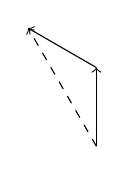
\begin{tikzpicture}
  \draw[->] (0,0)--(0,1);
  \draw[->] (0,1)--++({-cos(240+90)},{-sin(240+90)});
  \draw[dashed,->] (0,0) --({-cos(240+90)},{1-sin(240+90)});
\end{tikzpicture}
Векторное сложение МДС даст $\sqrt{3}$ при соединении обмоток в зигзаг,
а если соединить последовательно получилось бы увеличение в 2 раза.
\begin{tikzpicture}
  \draw[->] (0,0)--(0,1);
  \draw[->] (0,1)--++(0,1);
\end{tikzpicture}
В зигзаге получил примерно 15\% снижение возможного напряжения. Меди намотал на
200вольт, а получил 173вольта.
Одним из условий борьбы с вынужденным намагничиванием, чтобы ток протекал
в обе стороны. Из-за этого МДС будет направлена в разные стороны.

3-я схема. Ток протекает как нарисовано на схеме. Обмотки можно перевернуть
как в зигзаге
\begin{circuitikz}
\begin{scope}[xscale=0.8,yscale=0.8]\draw
  (0,0) to[L]++(0,1) node[right=2.4mm,below=0.6mm] {$\bullet$}
  (0.8,0) to[L]++(0,1) node[right=2.4mm,below=0.6mm] {$\bullet$}
  (1.6,0) to[L]++(0,1) node[right=2.4mm,below=0.6mm] {$\bullet$}
  %
  (0,1.2) to[L]++(0,1)
  (0,1.2) node[right=2.4mm,above=0mm] {$\bullet$}
  (0.8,1.2) to[L]++(0,1)
  (0.8,1.2) node[right=2.4mm,above=0mm] {$\bullet$}
  (1.6,1.2) to[L]++(0,1)
  (1.6,1.2) node[right=2.4mm,above=0mm] {$\bullet$}  
  ;\end{scope}\end{circuitikz}
можно не переворачивать
\begin{circuitikz}
  \begin{scope}[xscale=0.8,yscale=0.8]\draw
    (0,0) to[L]++(0,1) node[right=2.4mm,below=0.6mm] {$\bullet$}
    (0.8,0) to[L]++(0,1) node[right=2.4mm,below=0.6mm] {$\bullet$}
    (1.6,0) to[L]++(0,1) node[right=2.4mm,below=0.6mm] {$\bullet$}
    %
    (0,1.2) to[L]++(0,1) node[right=2.4mm,below=0.6mm] {$\bullet$}
    (0.8,1.2) to[L]++(0,1) node[right=2.4mm,below=0.6mm] {$\bullet$}
    (1.6,1.2) to[L]++(0,1) node[right=2.4mm,below=0.6mm] {$\bullet$}
    ;\end{scope}\end{circuitikz}.
Реактор здесь один -- $L$. Если ток течёт слева направо то половина вентилей
не работает. Вентильная группа $\textcyrillic{ВГ}_2$ обеспечивает протекание
тока в другую сторону. Ток по обмоткам трансформатора будет протекать в том же
направлении. В обратную сторону протекает ток обозначенный штриховкой.

1я схема) 2 набора обмоток и две вентильные группы. Каждый набор обмоток на
свою вентильную группу.

2я схема) Один набор обмоток на две группы вентилей.

3я схема)

\begin{tikzpicture}\draw
  (0,0.5) node {1й набор обмоток}
  (0,0) node {2й набор обмоток}
  (4.5,0.5) node {1я группа вентилей}
  (4.5,0) node {2я группа вентилей}  
  ;
  \draw[->] (1.7,0) -- (2.6,0);
  \draw[->] (1.7,0) -- (2.6,0.5);
  \draw[->] (1.7,0.5)  -- (2.6,0);
  \draw[->] (1.7,0.5) -- (2.6,0.5);
\end{tikzpicture}

Первая схема применялась с ионными вентилями. В то время применялись схемы с общим
катодом. Два бака катодов не применялось.
С тиристорными вентилями применялась вторая схема. Один комплект обмоток лучше чем
два.

Если считать что в каждом направлении машина работает 50мин - 1 час, то
считается что машина работает долго. Габариты удваиваются
$\displaystyle{\frac{S_1 + S_2}{2}}$. В длительном режиме суммарная мощность
трансформатора увеличивается в полтора раза. Сощность обмотки определяет расход
меди. Первичная обмотка всегда входит с коэффициэнтом 100\%.

$$
S_\textcyrillic{трансформатора} = \frac{S_1 + S_2}{2}
$$
Если в каждом направлении длительно работать, то
$S \approx 1.5 S_\textcyrillic{нагрузки}$, но так не говорят для постоянного тока,
говорят $=1.5  P_\textcyrillic{нагрузки}$

$[S] = V\!A(kV\!A)$, а мощность нагрузки киловатты
$S_\textcyrillic{трансформатора} = 1.5k P_\textcyrillic{нагрузки}$,
где $k$ зависит от коэффициэнта мощности и от ... (коэффициэнта формы?)

Если включение кратковременное м 50\% течёт и 50\% не течёт, то
среднеквадратичное включение $\displaystyle{\frac{1}{\sqrt{2}}}$
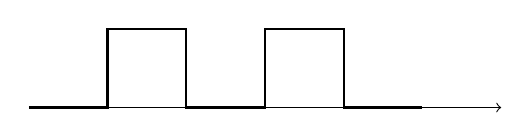
\begin{tikzpicture}
  \draw[thin,->] (0,0) -- (6,0);
  \draw[thick] (0,0)--(1,0)--(1,1)--(2,1)--(2,0)--(3,0)--(3,1)--(4,1)--(4,0)--(5,0);
  \end{tikzpicture}

$$
S_\textcyrillic{трансформатора} = \frac{1+2{\displaystyle \frac{1}{\sqrt{2}}}}{2}
\approx 1.205 k P_\textcyrillic{нагрузки}
$$

В любом случае в первой схеме больше потерь чем второй. Это главный недостаток
перекрёстной схемы. Третья схема: сделать выводы из трансформатора --
конструкция получается белее сложная.

Классификация по способу управления -- совместное управление группами вентилей
и раздельное управление группами вентилей.
Рассмотрим схему два. Ток не будет протекать справа -- раздельное управление.
По реализации оно сложнее. Включается инверторный режим, возникает опрокидывание.

Если не отключать вентили, а регулировать
$$
cos \alpha_1 + cos \alpha_2?
$$

\subsection{Эквивалентная схема замещения реверсивного тиристорного преобразователя}
\begin{circuitikz}\draw
  (0,5.6)--++ (0,-0.3)
  (0,4.8) circle (0.5cm)
  (0,4.8) node {$e_{d1}$}
  (0.5, 4.8) node[right] {$f(\alpha_1)$}
  (0,4.3)--++(0,-0.3)
  (0,1) to[battery1,l=$U_0$]++(0,1)
  to[L,l=$L_1$]++(0,1)
  to[R,l=$R_1$]++(0,1)
  (0,1) to[Do]++(0,-1)
%  --++(0,-0.5)
  %
  --++(3,0)
%  --++(0,0.5)
  to[Do,l=''VD'']++(0,1)
  to[battery1,l=$U_0$]++(0,1)
  to[L,l=$L_2$]++(0,1)
  to[R,l=$R_2$]++(0,1)
  --++(0,0.3)
  (3,4.8) circle (0.5cm)
  (3,4.8) node {$e_{d2}$}
  (3.5, 4.8) node[right] {$f(\alpha_2)$}
  (3,5.3)--++(0,0.3)
  %
  (3,0)--++(3,0)
  --++(0,0.5)
  (6,1) circle(0.5)
  (6,1) node {$E_\textcyrillic{н}$}
  (6,1.5)--++(0,0.5)
  to[L,l_=$L_\textcyrillic{н}$]++(0,1.5)
  to[R,l_=$R_\textcyrillic{н}$]++(0,2.1)
  --++(-6,0);
  %
  \draw[<-](-0.4,0.5)--++(-1.2,0) node[left] {идеальный диод};
  \draw[<-](2.4,0.2)--++(-1.5,-1) node[below] {все его параметры вошли в элементы выше выше}
  ;\end{circuitikz}

Вторая вентильная группа $U_0,L_2,R_2$

Предполагаем
$$
L_1=L_2=L
$$
$$
R_1=R_2=R
$$

$$
\underbrace{\displaystyle{}e_{d1}}_{\displaystyle \textcyrillic{мгновенное значение}}=
\overbrace{E_{d0}\;cos\alpha_1}^{
  \begin{array}{c}\textcyrillic{среднее значение}\\
    \textcyrillic{выпрямленного ЭДС}\end{array}} +
\underbrace{e_{d1\sim}}_{\displaystyle \textcyrillic{добавили пульсации}}
$$

$$
e_{d2} = E_{d0} \; cos \alpha_2 + e_{d2\sim}
$$

Чему равны $E_{d01}$ и $E_{d02}$ в первой схеме? Мы полагаем, что если $\alpha$ неодинаковые,
то пульсации неодинаковые.

Если раздельное управление?

А почему $\alpha$ разные.

\begin{circuitikz}\draw
  (0,1) to[Do] (0,0)
  (0,0) -- (1.4,0)
  (1.4,0) to[Do]++(0,1);
  \draw[->] (0.3,2)--(0.3,0.6) arc(180:360:0.4)--++(0,1.4);
  \draw (0,1.7) node {\it{i}};
\end{circuitikz}
Ток может протекать минуя нагрузку.


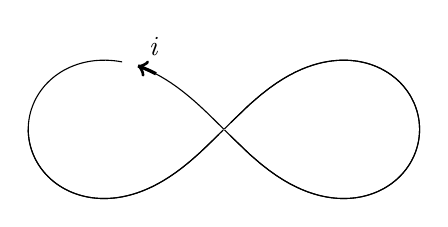
\begin{tikzpicture}[scale=10]
  \draw[thin,domain={-pi/4}:{pi/4},samples=100]
  plot (canvas polar cs:angle=\x r,radius=  {5*sqrt(2*cos(2*\x r))});
  \draw[thin,domain={pi-pi/4}:{pi-pi/4+0.15},samples=100]
  plot (canvas polar cs:angle=\x r,radius=  {5*sqrt(2*cos((-2*\x) r))});
  \draw[thin,domain={pi-pi/4+0.2}:{pi+pi/4},samples=100]
    plot (canvas polar cs:angle=\x r,radius=  {5*sqrt(2*cos((-2*\x) r))});
  \draw[thin,domain={pi/4}:{-pi/4},samples=100]
  plot (canvas polar cs:angle=\x r,radius=  {5*sqrt(2*cos(2*\x r))});
  \draw[thin,domain={pi+pi/4}:{pi},samples=100]
  plot (canvas polar cs:angle=\x r,radius=  {5*sqrt(2*cos((-2*\x) r))});
  % стрелка
  \draw[domain={pi-pi/4+0.1}:{pi-pi/4+0.15},samples=100,very thick,->]
  plot (canvas polar cs:angle=\x r,radius=  {0.02+5*sqrt(2*cos((-2*\x) r))})
  node[above right] {\it{i}};
  \end{tikzpicture}
В первой схеме протекает уравнительный ток, нежелательный, может быть неприемлимо
большой, аварийно-опасный.

%\begin{tikzpicture}[scale=2]
%  \draw[->] (-1,0) -- (1,0);
%  \draw[->] (0,-1) -- (0,1);
%  \draw node [red] at (-1,.25) {\scriptsize{Kardioida $r=5-5\sin \theta$}};
%  \draw[color=red,domain=0:6.28,samples=200,smooth]
%  plot (canvas polar cs:angle=\x r,radius={5-5*sin(\x r)});  %r = angle en radian
%  \end{tikzpicture} 

\begin{circuitikz}\draw
  (0,5.6)--++ (0,-0.3)
  (0,4.8) circle (0.5cm)
  (0,4.8) node {$e_{d1}$}
  (-0.3,5.3) node[left] {-}
  (-0.3,4.3) node[left] {+}
  (0.5, 4.8) node[right] {$\alpha=0$}
  (0,4.3)--++(0,-0.3)
  (0,1) to[battery1,l=$U_0$]++(0,1)
  to[L,l=$L_1$]++(0,1)
  to[R,l=$R_1$]++(0,1)
  (0,1) to[Do]++(0,-1)
  ;\end{circuitikz}
Условие отсутствия уравнительного тока $e_{d1}+e_{d2}\le 0!$ при пренебрежении $U_0$.

$e_{d1}+e_{d2}\le 2U_0$

$$
E_{d0} (cos \alpha_1 + cos \alpha_2) + e_\textcyrillic{уравнительное} \le 2U_0
$$
где $e_\textcyrillic{уравнительное} = e_{d1\sim} + e_{d2\sim}$

Можно записать отдельно условия отсутствия уравнительного тока:

Переменная составляющая уравнительного тока должна быть $\le 2U_0$ и
постоянная составляющая уравнительного тока должна быть $\le 2U_0$.

Для постоянной составляющей
$$
E_{d0} (cos \alpha_1 + cos \alpha_2)\le 2U_0 \Rightarrow cos \alpha_1 + cos \alpha_2
\le \frac{2U_0}{E_{d0}}
$$

Если $\displaystyle \frac{2U_0}{E_{d0}}\approx 0$ тогда пишем для случая равенства 0:

$$
  \bcancel{2}cos\frac{\alpha_1 +\alpha_2}{2}\cdot cos \frac{\alpha_1 -\alpha_2}{2} \le 0
$$

$$
  \begin{array}{c}
    0<\alpha_1<\pi-\xcancel{\beta_{min}}\\
    0<\alpha_2<\pi-\xcancel{\beta_{min}}
    \end{array}
$$
  
но $\displaystyle cos \frac{\alpha_1-\alpha_2}{2}\ne 0$ никогда не равно нулю на всем
  диапазоне.

  \begin{equation}
    cos \frac{\alpha_1+\alpha_2}{2}\le 0
  \end{equation}

  $$
  E_{d0}(cos \alpha_1+ cos\alpha_2)\le2U_0
  $$
  \begin{equation}\left\{\begin{array}{ll}
      \alpha_1+\alpha_2\ge\pi&
        {\displaystyle\textcyrillic{ ( при} \frac{U_0}{E_{d0}}=0)}\\
      {\displaystyle cos\; \alpha_1+ cos\;\alpha_2 \le \frac{2U_0}{E_{d0}}}&
    \end{array}\right.
\label{codrive}
  \end{equation}
  Условия  (\ref{codrive}) являются условиями совместного управления.
  $\alpha_1$ меняется, чтобы вторая группа не мешала $\alpha_1=\pi-\alpha_2$

  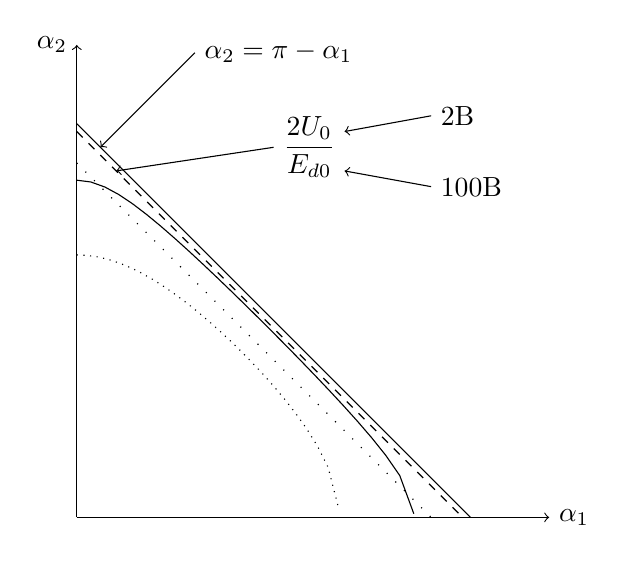
\begin{tikzpicture}
    \begin{scope}[scale=1]
      \draw[thin,->] (0,0) -- (6,0) node[right] {$\alpha_1$};
      \draw[thin,->] (0,0) -- (0,6) node[left] {$\alpha_2$};
    \draw[domain=0:5]
    plot (\x,5-\x);
    \draw[dashed,domain=0:4.9]
        plot (\x,5-\x-0.1);
    \draw[domain=0:4.28]
    plot (\x, {acos( (0.1-cos((\x*pi/5) r)) )/180*5 });
    % 2U_0/E_d0 = 0.5/5
    \draw[loosely dotted,domain=0:4.5]
        plot (\x,5-\x-0.5);
    \draw[dotted,domain=0:3.33]
    plot (\x, {acos( (0.5-cos((\x*pi/5) r)) )/180*5 });
    \draw[thin,<-] (0.3,{5-0.3}) -- (1.5,5.9) node[right] {$\alpha_2 = \pi - \alpha_1$};
    \draw[<-] (0.5,{5-0.5-0.1}) -- (2.5,4.7) node[right]
         {$\displaystyle{\frac{2U_0}{E_{d0}}}$};
    \draw[thin,<-] (3.4,4.9) -- (4.5,5.1) node[right] {2B};
    \draw[thin,<-] (3.4,4.4) -- (4.5,4.2) node[right] {100B};
    \end{scope}
  \end{tikzpicture}  

  Регулируем напряжение на нагрузке.

  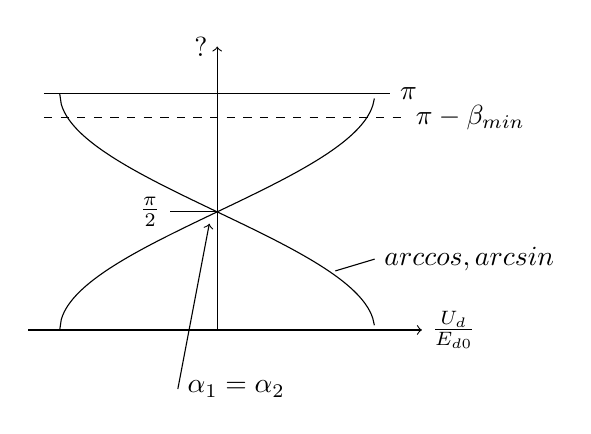
\begin{tikzpicture}
    \begin{scope}[xscale=2,yscale=3]
      \draw[thin,->] (-1.2,0) -- (1.3,0) node[right] {$\frac{U_d}{E_{d0}}$};
      \draw[thin,->] (0,0) -- (0,1.2) node[left] {?};
      \draw[thin] (-1.1,1) -- (1.1,1) node[right] {$\pi$};
      \draw[thin,dashed] (-1.1,0.9) -- (1.2,0.9) node[right] {$\pi-\beta_{min}$};
      \draw[domain=-1:1,samples=200]
      plot(\x, {acos(\x)/180});
      \draw[domain=-1:1,samples=200]
      plot(\x, {asin(\x)/180+0.5});
      %
      \draw[thin] (0,0.5) -- (-0.3,0.5) node[left] {$\frac{\pi}{2}$};
      \draw[thin] (0.75,0.25) -- (1,0.3) node[right] {$arccos,arcsin$};
      \draw[thin,<-] (-0.05,0.45) -- (-0.25,-0.25) node[right] {$\alpha_1= \alpha_2$};
    \end{scope}
  \end{tikzpicture}

  Получили соотношение для постоянных составляющих при совместном управлении.

  $$
  e_{d1\sim} + e_{d2\sim} = U_\textcyrillic{ур} \le 0
  $$
  Корректно ли ставить такую задачу? переменная составляющая на самом деле --
  знакопеременная. Уравнительный ток останется. Если ток переменный, то его можно
  ограничить индуктивностью до заранее выбранного значения.

  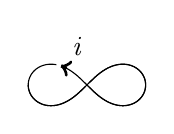
\begin{tikzpicture}[scale=3]
    \draw[thin,domain={-pi/4}:{pi/4},samples=100]
    plot (canvas polar cs:angle=\x r,radius=  {5*sqrt(2*cos(2*\x r))});
    \draw[thin,domain={pi-pi/4}:{pi-pi/4+0.15},samples=100]
    plot (canvas polar cs:angle=\x r,radius=  {5*sqrt(2*cos((-2*\x) r))});
    \draw[thin,domain={pi-pi/4+0.2}:{pi+pi/4},samples=100]
    plot (canvas polar cs:angle=\x r,radius=  {5*sqrt(2*cos((-2*\x) r))});
    \draw[thin,domain={pi/4}:{-pi/4},samples=100]
    plot (canvas polar cs:angle=\x r,radius=  {5*sqrt(2*cos(2*\x r))});
    \draw[thin,domain={pi+pi/4}:{pi},samples=100]
    plot (canvas polar cs:angle=\x r,radius=  {5*sqrt(2*cos((-2*\x) r))});
    % стрелка
    \draw[domain={pi-pi/4+0.1}:{pi-pi/4+0.15},samples=100,very thick,->]
    plot (canvas polar cs:angle=\x r,radius=  {0.02+5*sqrt(2*cos((-2*\x) r))})
    node[above right] {\it{i}};
  \end{tikzpicture} -- переменная составляющая 50-70\%. Что можно сделать?

  Иногда делают навстречу постоянное напряжение
  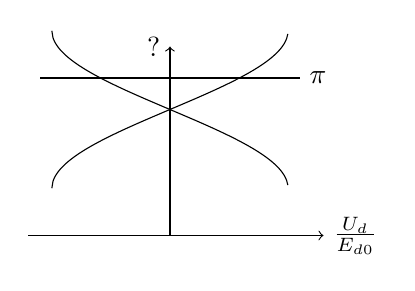
\begin{tikzpicture}
    \begin{scope}[xscale=1.5,yscale=2]
      \draw[thin,->] (-1.2,0) -- (1.3,0) node[right] {$\frac{U_d}{E_{d0}}$};
      \draw[thin,->] (0,0) -- (0,1.2) node[left] {?};
      \draw[thin] (-1.1,1) -- (1.1,1) node[right] {$\pi$};
%      \draw[thin,dashed] (-1.1,0.9) -- (1.2,0.9) node[right] {$\pi-\beta_{min}$};
      \draw[domain=-1:1,samples=200]
      plot(\x, {0.3+acos(\x)/180});
      \draw[domain=-1:1,samples=200]
      plot(\x, {0.3+asin(\x)/180+0.5});
    \end{scope}
  \end{tikzpicture}

  Для ограничения уравнительного тока обусловленного переменной составляющей
  уравнительного тока используются уравнительные реакторы.

  Схему иногда называют ''восьмеркой''. Как расчитать реакторы? Существуют графики,
  можно определить зависимость от одного угла, либо от выпрямленного напряжения.
  Ток переменный или постоянный. Пойдёт ток как в однополупериодной схеме.
  
  \begin{circuitikz}\draw
    (0,1) to[Do] (0,0)
    (0,0) -- (1.4,0)
    (1.4,0) to[Do]++(0,1);
  \end{circuitikz} -- однополупериодная схема.

  Если ток течёт без перерыва, то падение напряжения $U=0$.
  $I_\textcyrillic{малый ток}\cdot r_\textcyrillic{проводов}$ -- величина второго
  порядка малости если обеспечен $I_\textcyrillic{малый ток}$.

  Зависимость $U_\textcyrillic{выпрямленного}$ от $\alpha$.

  Задавшись максимальным уравнительным током $\Rightarrow$ зададимся индуктивностью.
  Ток загружает вентили, загружает трансформатор.
  Используемые уравнительные реакторы выбираются по максимальному значению
  $U_\textcyrillic{ур.}$, зависящему от соотношения углов $\alpha$. Обычно
  величина $I_\textcyrillic{ур.}$ ограничивается на 10\% меньше от номинального
  $I_\textcyrillic{выпрямленного}$

  Как протекает ток в схеме 2
  \begin{circuitikz}\draw
    (1,3) to[L,l=$A$] (1,2)--(0,2)--(0,0)
    to[L] (1,0) --(2,0) to[L](3,0)--(3,2)--(2,2)--(2,3) to[L,l=C] (2,4)
;    \end{circuitikz}
  Ток из одной фазы переходит в другую.
  В тертьей схеме
  \begin{circuitikz}\draw
    (1,5)--(1,4)to[short,l=A](0,4)--(0,2)to[short,l=B](1,2)--(1,0)--(3,0)to[L,l=$L$](3,2)
    (0,2)--(0,1)to[short,l=C](1,1)
    ;\end{circuitikz}
  существует два контура уравнительного тока, а реактор один для двух контуров тока.
  H-схема -- средняя. Вторая схема самая хорошая. Фирмы-производители не часто
  использовали H-схему.

  Для мостовой схемы зигзаг не нужен.
  
  \begin{circuitikz}\begin{scope}
    \draw
  (1,1) to[Ty] (2,1) -- (4,1) to[Ty,*-] (5,1)--(5,2)
  (1,1)--
  (1,2) to[Ty] (2,2) -- (3,2)--(4,2) to[Ty] (5,2)--(5,3)
  (1,2)--
  (1,3) to[Ty,-*] (2,3) -- (4,3) to[Ty] (5,3)
  %
  (5,4) to[Ty,-*] (4,4)--(2,4) to[Ty] (1,4)--(1,5)
  (5,4)--
  (5,5) to[Ty] (4,5)--(2,5) to[Ty] (1,5)--(1,6)
  (5,5)--
  (5,6) to[Ty] (4,6)--(2,6) to[Ty,*-] (1,6)
  %
  (2,3)--(2,8)
  (3,2)to[short,*-*](3,5)--(3,8)
  (4,1)--(4,8)
  %
  (2,8)to[L,l=A](2,9.3)--(2.4,9.3)--(2.4,8)--(3,8)
  (3,8)to[L,l=B](3,9.3)--(3.4,9.3)--(3.4,8)--(4,8)
    
    %уравнительные реакторы
    (1,2)--(0,2)--(0,2.5) arc(90:-180:0.5)--(-1,2)
    (-0.4,2.1) node[above] {$L_2$}
    (1,5)--(0,5)--(0,5.5) arc(90:-180:0.5)--(-1,5)
    (-0.4,5.1) node[above] {$L_1$}
    %
    (5,2)--(6,2)--(6,2.5) arc(90:360:0.5)--(7,2)
    (6.4,2.1) node[above] {$L_4$}
    (5,5)--(6,5)--(6,5.5) arc(90:360:0.5)--(7,5)
    (6.4,5.1) node[above] {$L_3$}
    %к мотору
    (-1,5)to[short,-*](-1,2)--(-1,0)--(2.5,0)
    (7,5)to[short,-*](7,2)--(7,0)--(3.5,0)
    %мотор
    (3,0) circle (0.5cm)
    (3,0) node {M}
    %core трансформатора
    (2,9.49) rectangle (4,9.51)
    %LLL
    (2,9.7)to[L](2,11)
    (3,9.7)to[L](3,11)
    (4,9.7)to[L](4,11)
    (2,9.7)--(4,9.7)
    
    %рисуем ток
    (1.4,6.5) node {$\leftarrow A$}
    (2.4,2.3) node {$B\rightarrow$}
    ;
    % рисуем ток КЗ при коммутации
    \draw[dotted,color=red,->] (1.9,6.1)--(1,6.1)arc(90:180:0.1)--(0.9,5.5)
    arc(0:-90:0.4)--(-0.3,5.1)arc(90:180:0.6)--(-0.9,2.7)arc(180:270:0.6)--
    (0.5,2.1)arc(270:360:0.4)--(0.9,3)arc(180:90:0.1)--(1.4,3.1)arc(270:360:0.5)
    --(1.9,5.8);
    \draw[dotted,color=red,<-] (-1,3.6)--(-1.5,-1) node[right]
         {часть периода при коммутации будет течь ток К.З.};
   %
  \draw[dotted] (4.1,8.1)to[L,l=C](4.1,9.4)--(4.5,9.4)--(4.5,8.1)--(5.1,8.1);
  \draw[thin,<-] (4.5,8.7) -- (6,9) node[right]
       {$\begin{array}{c}\textcyrillic{чтобы подчеркнуть,}\\
           \textcyrillic{что средняя точка не нужна}\\
\textcyrillic{и обмотка C не нужна!}
         \end{array}$};
    \end{scope}
\end{circuitikz}  

  Куда включить реакторы? Сначала включим по самой сложной/полной схеме. Потом будем
  выбрасывать. $\cancel{L_2}\cancel{L_3}$ -- можно убрать два реактора, только
  симметрично. Могут использоваться 2 реактора или все четыре. Наличие двух
  контуров уравнительного тока с большой составляющей переменного напряжения
  является главным недостатком встречно-параллельной схемы.

  \begin{circuitikz}\draw
    (4,2)to[Ty](3,2)--(1,2)to[Ty](0,2)
    (4,3)to[Ty](3,3)--(1,3)to[Ty](0,3)
    (4,4)to[Ty](3,4)--(1,4)to[Ty](0,4)
    %
    (10,2)to[Ty](9,2)--(7,2)to[Ty](6,2)
    (10,3)to[Ty](9,3)--(7,3)to[Ty](6,3)
    (10,4)to[Ty](9,4)--(7,4)to[Ty](6,4)
    %
    (0,4)--(0,0)--(1,0)to[L,l=$\textcyrillic{Ур}_1$](2,0)--(5,0)--(8,0)
    to[L,l=$\textcyrillic{Ур}_2$](9,0)--(10,0)--(10,4)
    % средняя точка моста
    (4,2)--(4,4)
    (6,2)--(6,4)
    (4,3)--(6,3)
    %LLL LLL
    (1,4)to[short,*-]++(0,1)to[L](1,6.3)
    (2,3)to[short,*-]++(0,2)to[L](2,6.3)
    (3,2)to[short,*-]++(0,3)to[L](3,6.3)--++(-2,0)   
    %
    (7,4)to[short,*-]++(0,1)to[L](7,6.3)
    (8,3)to[short,*-]++(0,2)to[L](8,6.3)
    (9,2)to[short,*-]++(0,3)to[L](9,6.3)--++(-2,0)

    %мотор
    (5,0)to[short,*-](5,1)
    (5,2)to[short,-*](5,3)
    (5,1.5) circle (0.5cm)
    (5,1.5) node {M}
    
    %core
    (1,6.49) rectangle (9,6.51)
    % LLL первичная сторона
    (4,6.7)to[L]++(0,1.3)
    (5,6.7)to[L]++(0,1.3)
    (6,6.7)to[L]++(0,1.3)
    (4,6.7)--(6,6.7)
    ;\end{circuitikz}
  
  Выбор уравнительного напряжения -- по амплитуде.
  6-ти пульсная схема + 6-ти пульсная = пульсации меньше. А в предыдущей схеме 3-х
  пульсная (4 реактора,мощность на большую амплитуду и низкую частоту) H-схема
  имеет преимущество, потому что один реактор.

  При раздельном управлении
  импулься поступают на одну ... Необходимость использования уравнительных реакторов
  отсутствует. По этому признаку можем отличить раздельное управление.

  По сравнению с предыдущей схемой
  
  \begin{circuitikz}\draw
    % средняя точка моста
    (4,2)--(4,4)
    (6,2)--(6,4)
    (4,3)--(6,3)
    
    %мотор
    (5,0)to[L,*-](5,1)
    (5,2)to[L,-*](5,3)
    (5,1.5) circle (0.5cm)
    (5,1.5) node {M}
    %
    (2,0)--(8,0)
    ;
    \draw[thin,<-] (5.4,0.5)--(6.4,2) node[right]
         {$\begin{array}{c}\textcyrillic{сглаживающие реакторы}\\
             \textcyrillic{ставим здесь или здесь}\end{array}$};
    \draw[thin,<-] (5.4,2.5)--(6.4,2);
  \end{circuitikz}
  
  Отсутствие уравнительных токов и отсутствие реакторов является главным достоинством
  раздельного способа управления.

  Если один выпрямитель а другой инвертор сумма углов 180.
  $$
  \begin{array}{cc}
    \alpha=60 & \alpha=120\\
    cos = \frac{1}{2} &  cos = -\frac{1}{2}
    \end{array}
  $$

  В схеме замещения:
 \begin{circuitikz}\draw
    (0,1) to[Ty] (0,0) -- (2,0) to[Ty] (2,1)
    (0,1.5) node{+}
    (0,2) node{-}
    (2,1.5) node{+}
    (2,2) node{-}
    (0,-0.6)node{напряжение $\frac{1}{2}$ и $\frac{1}{2}$}
    ;\end{circuitikz}

 А как протекает ток? агрузка выбирает куда течь току. Возникает полная аналогия
 с системой Леонардо(генератор+двигатель)
 
 \begin{circuitikz}\draw
   (0,0)circle(0.5)
   (0,0)node{M}
   (0,-0.7)node{противо ЭДС}
   (0,2)circle(0.5)
   (0,2)node{G}
   (-0.5,0)--(-1,0)--(-1,2)--(-0.5,2)
   (0.5,0)--(1,0)--(1,2)--(0.5,2)
   ;\end{circuitikz}   
 
 Двигатель выбирает направление тока.

 Обмоткой возбуждения можно заставить ...

 Недостаток раздельного управление ... ток не протекает ... но из-за управл.

 Плохо, что всегда есть инвертор. потому что принципиально инвертор ненадежен.
 Инверторный двигатель не в состоянии выбрать направление.

 Второй недостаток схемы совместного?? управления -- всегда имеет инверторный режим.
 Достоинство = полная идентичность с системой двигатель+генератор
 

 А при раздельном управлении нужно соответствующее управление.

 Как реализовать раздельное управление?

 \subsection{Принципы построения раздельной системы управления}

 \begin{circuitikz}\draw
   (0,5.6)--++ (0,-0.3)
   (0,4.8) circle (0.5cm)
   (0,4.8) node {$e_{d1}$}
   (-0.5, 4.8) node[left] {$\alpha_1\rightarrow$}
   (0,4.3)--++(0,-0.3)
   (0,1) to[battery1,l=$U_0$]++(0,1)
   to[L,l=$L_1$]++(0,1)
   to[R,l=$R_1$]++(0,1)
   (0,1) to[Do]++(0,-1)
   %  --++(0,-0.5)
   %
   --++(3,0)
   %  --++(0,0.5)
   to[Do]++(0,1)
   to[battery1,l=$U_0$]++(0,1)
   to[L,l=$L_2$]++(0,1)
   to[R,l=$R_2$]++(0,1)
   --++(0,0.3)
   (3,4.8) circle (0.5cm)
   (3,4.8) node {$e_{d2}$}
   (1.5, 4.8) node[right] {$\alpha_2\rightarrow$}
   (3,5.3)--++(0,0.3)
   %
   (3,0)--++(3,0)
   --++(0,0.5)
   (6,1) circle(0.5)
   (6,1) node {$E_\textcyrillic{н}$}
   (6,1.5)--++(0,0.5)
   to[L,l_=$L_\textcyrillic{н}$]++(0,1.5)
   to[R,l_=$R_\textcyrillic{н}$]++(0,2.1)
   --++(-6,0);
   %
   ;\end{circuitikz}
 
 При переходе к раздельному управлению технологи не торопились снимать уравнительные реакторы.
 Инерционность реакторов помогала защите.

 При переключении вентильных групп
 \begin{enumerate}
 \item вначале выключаются импульсы одной вентильной группы, затем включаются на другой;
 \item отключать можно в тот момент когда ток равен нулю. Потому что пока есть ток
   есть инверторный режим нельзя включать. Включение при нулевом токе в нагрузке.
 \item после того как ток спал до нуля, но включать только после паузы превышающей
   время выключения вентилей
 \end{enumerate}

 \begin{enumerate}
 \item вначале отключили, потом включили
 \itemотключение после того как ток $I=0$
 \item выключение спустя $\scriptstyle{\Delta}t >t_\textcyrillic{выключение тиристора}$.
   Есть дополнительное условие: нельзя отключать импульсы в момент формирования импульсов
 \item тиристор открылся а датчик не смог ... определить что ток есть. Запрет отключения
   в момент когда импульс сформировался.
 \item (замена второго пункта, вариант) Вместо контроля за током используется контроль
   состояния всех тиристоров(вентилей)   
 \end{enumerate}

 $10kA$, чтобы гарантировать что тиристоры выключились, $I<I_\textcyrillic{удержания}$,
 100-200mA. Покажет ток утечки тиристоров, а этот ток может быть большим, потому что
 используется несколько тиристоров.
 Ток утечки 18 закрытых тиристоров может быть больше чем ток удержания одного тиристора.
 Определив ток, не знаем что эо за ток: ток удержания одного тиристора или ток утечки всех.

 Датчики ДЗВ (запирания вентилей). Будем контролировать
 $\scriptstyle{\Delta}U_\textcyrillic{тиристора}$. 15 вольт -- гарантия что тиристор заперт.
 На каждом больше 15 вольт -- точно заперт
\begin{figure}[H]
 \begin{tikzpicture}
   \draw[thin,->] (-pi/2,0) -- (3*pi/2+pi/2,0) node[right] {$\omega t$};
   %
   \draw[domain=-pi/2:pi/2]
   plot (\x,{cos(\x r)});
   \draw[domain={0+pi/6}:{pi+pi/6}]
   plot (\x,{cos((\x-pi/2-pi/6) r)});
   \draw[domain={pi/2+pi/3}:{3*pi/2+pi/3}]
   plot (\x,{cos((\x-pi-pi/3) r)});
   % скобки
   \draw[red,thin] (pi/6-0.15,-0.2)--(pi/6-0.15,0.2) (pi/6+0.15,-0.2)--(pi/6+0.15,0.2);
   \draw[thin,<-] (pi/6,0) -- (pi/6,-0.6) node[below] {зоны ложного запрета};
   % отрезки на кривых
   \draw[red,domain={pi/2-0.2}:{pi/2+0.2},very thick]
   plot (\x,{cos(\x r)+0.05});
   \draw[red,domain={pi/2+pi/3-0.2}:{pi/2+pi/3+0.2},very thick]
   plot (\x,{cos((\x-pi-pi/3) r)+0.05});
   \end{tikzpicture}
\end{figure}
Тиристор открыт -- на нем нуловое напряжение. Лучше ложный запрет чем ложное разрешение.

НПЧ -- непосредственный преобразователь частоты.
 
